\documentclass[14pt,a4paper]{extarticle}

\usepackage{fontspec}
\IfFontExistsTF{Times New Roman}{\setmainfont{Times New Roman}}{\setmainfont{Liberation Serif}}
\usepackage{graphicx}
\usepackage{float}
% на машине без пакета babel-russian используется описание языка из babel
\IfFileExists{russianb.ldf}{\usepackage[russian]{babel}}{\usepackage{babel}\babelprovide[import,main]{russian}}
\usepackage[a4paper, left=30mm, right=15mm, top=20mm, bottom=20mm]{geometry}
\usepackage{setspace}
\usepackage{indentfirst}
\usepackage{titlesec}
\usepackage{amsmath}
\graphicspath{{figures/}}

\setstretch{1.2}
\setlength{\parindent}{1.25cm}
\setlength{\emergencystretch}{3em}

\begin{document}
	\begin{titlepage}
		\thispagestyle{empty}
		\begin{center}
			\vspace{1cm}
			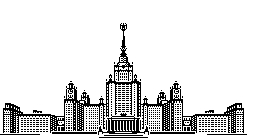
\includegraphics[width=10cm]{mgu.jpg} \\
			Московский государственный университет имени М.\,В.~Ломоносова\\
			Факультет вычислительной математики и кибернетики\\
			Кафедра вычислительных методов
		\end{center}
		
		\vspace{2cm}
		
		\begin{center}
			{\large Дю Василий Андреевич}
		\end{center}
		
		\vspace{2cm}
		
		\begin{center}
			{\bfseries\large МОДЕЛИРОВАНИЕ ОДНОЙ ДИФФЕРЕНЦИАЛЬНОЙ ИГРЫ\\}
		\end{center}
		
		\vspace{1.8cm}
		
		\begin{center}
			{\large КУРСОВАЯ РАБОТА}
		\end{center}
		
		\vfill
		
		\begin{flushright}
			Научный руководитель:\\
			к.ф.-м.н., доцент\\
			В.\,В.~Терновский
		\end{flushright}
		
		\vfill
		
		\begin{center}
			Москва, 2026
		\end{center}
		
	\end{titlepage}
	\tableofcontents
	\newpage
	\section{Введение}
	
	Дифференциальные игры представляют собой важный раздел современной теории управления, в котором рассматриваются конфликтные процессы с участием двух и более сторон. Особый интерес вызывают задачи преследования и уклонения, поскольку они находят применение в математическом моделировании, робототехнике, экономике и военных приложениях.
	
	Одной из классических моделей такого типа является дифференциальная игра «шофёр--убийца», предложенная Р.~Айзексом~\cite{isaacs}. В данной работе рассматриваются основные подходы к постановке этой игры, математическая модель движения участников, а также особенности численного моделирования траекторий.
	
	\section{Постановка задачи}
	
	В играх преследования используются обозначения преследователя как P, преследуемого объекта как E. Соответствующие движущиеся объекты могут управляться как человеком, так и автоматически. В более сложных задачах рассматривается более двух <<игроков>>, например группа преследователей и группа преследуемых объектов. В общем случае P и E противники с противоположными интересами которые могут применять любые управления допустимые в соответствии с заданной динамикой процесса. Игра преследования вообще говоря заканчивается когда расстояние между P и E стало меньше некоторой заранее заданной величины. Для пояснения идей нужно понимать следующие пункты: Возможно ли окончание игры, пояснение оптимальные стратегии для P и для E в совокупности, т.е как они должны изменять свои управления в каждый момент времени зная свои фазовые координаты , а также фазовые координаты противника. Во вторых, для игры нужно поставить плату. Например для задачи, где захват объекта E неизбежен, критерий или плата наиболее очевидна. Как пример такой платы можно взять либо расстояние которое обьекты преодолели до захвата, либо же в нашей задаче плата времени захвата. Игра <<шофёр--убийца>> происходит на плоскости, где преследователь P движется с фиксированной скоростью w1, а радиус кривизны траектории ограничен заданным радиусом R; При этом P может управлять радиусом. Убегающий (пешеход) обладает более простым движением и, соответственно, управлением. Скорость w2 фиксирована, и управление состоит в выборе направления движения.
	
	\section{Математическая модель}
	
	\subsection{Кинематика}
	Место действия представляет собой $\ell$-область в $n$-мерном евклидовом пространстве и её границу. Система дифференциальных уравнений имеет вид
	\[
	\dot{x}_i = f_i\bigl(x_1, \dots, x_n, \phi_1, \dots, \phi_\lambda, \psi_1, \dots, \psi_\kappa\bigr),
	\]
	описывающий движение некоторой точки
	\[
	x(t) = \bigl(x_1, x_2, \dots, x_n\bigr).
	\]
	или короче можно задать в виде
	\[
	\dot{x}(t) = f\bigl(x(t), \phi(t), \psi(t)\bigr),
	\]
	функции $f_i$ заданы. Мы предполагаем их достаточно гладкими, так что существуют все их частные производные, которые нам в дальнейшем понадобятся. 
	\begin{figure}[H]
		\centering
		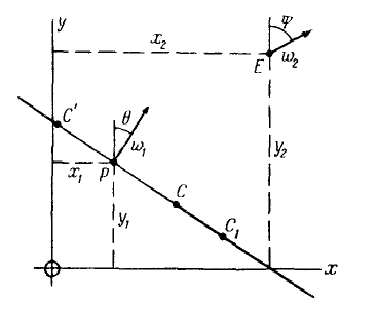
\includegraphics[width=0.8\textwidth]{dynamic.png}
		\caption{Описательная динамика движения P и E}
\label{fig:full-dynamics}
	\end{figure}
	Переменные $\phi$, $\psi$ называем управлениями. P и E могут изменять их в любой момент времени. На $\phi$ и $\psi$ есть ограничения. Эти ограничения задают векторограмму для P и для E в пространстве $\ell$ при фиксированных $\psi$ и x или $\phi$ и x. А полной векторограммой будем называть векторограмму, которая пробегается по всем значениям $\phi$ и $\psi$. Перейдём теперь к уравнениям движения для нашей дифференциальной игры. Для записи данного уравнения достаточно задать 5 фазовых координат; по две координаты для обозначения P и 2 для E. $x_1$, $y_1$, $x_2$, $y_2$ а также параметр $\theta$
	Управление для E выглядит проще. Для описания направления его движения задается вектор $\psi$. Управление для P выглядит немного сложнее. В произвольный момент времени P волен выбирать мгновенный центр кривизны своей траектории в любой точке например на картинке $C_1$, лежащий на этой прямой вне интервала C'C. Управление $\phi$ будем считать равным по модулю величине R/|P$C_1$| положительным для точек $C_1$, лежащих справа от P, и отрицательным - слева. Таким образом -1 $\leq$ $\phi$ $\leq$ 1. Тогда уравнение движения выглядит следующим образом:
	\[\dot{x_1} = w_1 \sin(\theta)\]
	\[\dot{y_1} = w_1 \cos(\theta)\]
	\[\dot{x_2} = w_2 \sin(\psi)\]
	\[\dot{y_2} = w_2 \cos(\psi)\]
	\[\dot{\theta} = w_1 \phi / R \]
	
	\subsection{Редуцированное пространство}
	
	Перейдем к рассмотрению редуцированного пространства для задачи Шофер убийца. Разберем как можно перейти от модели построенной на кинематике к системе меньшей размерности, чтобы можно было получить непосредственное и исчерпывающее описание ситуации. Однако число n, размерность пространства $\ell$, может оказаться для этого излишне большим. Как и в нашей задаче. В задаче шофер-убийца допустимо понижение размерности с 5 фазовых координат до 2. Для этого достаточно поместить начало новой системы координат в точку P и направить ось $y$ по направлению движения P. 
	
	\begin{figure}[H]
		\centering
		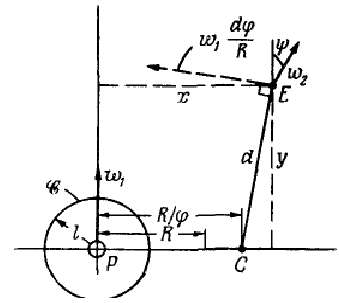
\includegraphics[width=0.8\textwidth]{reduced_dynamic.png}
		\caption{Редуцированная динамика движения P и E}
\label{fig:reduced-dynamics}
	\end{figure}
	
	Вращение P вокруг C эквивалентно вращению x вокруг C в противоположном направлении, но с той же угловой скоростью. x движется со скоростью по модулю равную $w_1$(d$\phi$/R) в направлении перпендикулярном CE. Составляющие его скорости получаются умножением модуля соответственно на -y/d и (x-R/$\phi$)/d Уравнения движения в редуцированном пространстве имеют вид: 
	\[\dot{x} = -w_1/R * y\phi + w_2\sin(\psi)\]
	\[\dot{y} = w_1/R * x \phi - w_1 + w_2\cos(\psi);     -1 \leq \phi\ \leq 1\]
	
	\subsection{Окончание игры}
	
	Имеется некоторая поверхность \( \mathcal{E} \), называемая терминальной поверхностью и представляющая собой часть границы пространства \( \ell \). Когда \( x \) достигает \( \mathcal{E} \), игра оканчивается.
	Почему поверхность?
	Игра преследования обычно заканчивается захватом, который на первый взгляд должен состоять в совпадении точек \( P \) и \( E \). Однако:
	\begin{itemize}
		\item Это нереально: \( P \) и \( E \) — фиксированные точки на реальных объектах (самолёт, корабль, торпеда) и никогда не совпадут.
		\item В тактических ситуациях достаточно близости, а не контакта.
	\end{itemize}
	Поэтому разумный критерий захвата: задать положительное число \( l \) и считать, что захват происходит, когда расстояние между \( P \) и \( E \) равно \( l \). Множество всех точек захвата описывается одним уравнением, следовательно, оно представляет собой поверхность.
	
	Случай, когда \( \mathcal{E} \) внутри пространства
	Если \( \mathcal{E} \) находится не на границе, а внутри \( \ell \), то она разделяет пространство на две стороны. Часто окончанием игры считаются только те случаи, когда \( x \) достигает \( \mathcal{E} \) с определённой стороны.
	
	Параметризация терминальной поверхности
	Поскольку \( \mathcal{E} \) является \( (n-1) \)-мерным многообразием, выразим её через \( n-1 \) параметр:
	\[
	x_i = h_i(s_1, \dots, s_{n-1}) = h_i(s), \quad i = 1, \dots, n.
	\]
	Функции \( h_i \) предполагаются дифференцируемыми (в худшем случае — кусочно-гладкими; тогда каждый кусок рассматривается отдельно).
	
	\subsection{Плата}
	Теперь поговорим про плату. Данную численную величину, которую игроки стараются минимизировать или максимизировать в играх степени, может иметь различный вид. Как плату мы берем за образец следующую форму платы:
	\[\int G(x, \phi, \psi)dt + H(s)\] 
	Будем предполагать, что функция G, так же как $f_i$, обладает частными производными. Интеграл берется вдоль траектории, которую x проходит в $\ell$ на протяжении партии где нижний предел можно взять равным 0, а верхний --- временем окончания игры. В игре <<шофёр--убийца>> рассматривается игра на время: $G\equiv 1$, $H=0$, т.\,е. плата равна времени до захвата.
	
	\subsection{Техника решения}
	Эта часть будет рассматривать следующие вопросы:
	\begin{enumerate}
		\item Цена игры V(x) определенная на $\ell$
		\item Оптимальные стратегии: вектор функции $\overline{\phi}$, $\overline{\psi}$
		\item Оптимальные траектории
	\end{enumerate}
	Процесс решения игры распадается на 2 фазы. В основном оказывается что область $\ell$ подразделяется на области, которые разделяются сингулярными поверхностями, которые нарушают гладкость или определенность. Собственно в данных областях решение будет гладким, так что V принадлежит классу $C^1$. Геометрически это означает, что поверхности постоянных значений V имеют непрерывно меняющиеся касательные плоскости. В силу непрерывности функции справедливо что для достаточно малых значений вектора u = ($u_1$, $\dots$, $u_n$) справедливо:
	\[
	V(x + u) - V(x) = \sum_{i=1}^{n} \frac{\partial V(x)}{\partial x_i}\, u_i + o(|u|)
	\]
	На сингулярных поверхностях как до этого было сказано могут возникать особенности разных типов. Техника нахождения решения в малых частях между сингулярных поверхностях ничем не отличается от техники решений дифференциальных уравнений. Но не все типы сингулярных поверхностей допускают классический подход вариационного исчисления. Игра шофер убийца относится к типу игр, где решение между сингулярными поверхностями просты, но эти сингулярные поверхности многочисленны и многообразны.
	Теперь поговорим про принцип перехода. Он формулируется так: Если в игре произошел переход из одного положение в другое и если во втором положении известно значение V, то в первом оно определяется следующим требованием: игроки должны оптимизировать приращение функции V(добиться его минимакса) за время перехода. 
	\[
	\min_{\varphi} \max_{\psi} \left[ \sum_{j=1}^{n} V_j f_j(x, \varphi, \psi) + G(x, \varphi, \psi) \right] = 0
	\]   
	Суть данного уравнения состоит в том, что рассматривается совокупность траекторий исходящих из различных точек. Тогда возьмем фиксированное значение t в этой игре и пусть значение V в данной точке известно. Тогда для достаточного маленького h - промежуток времени положение изменится и мы перейдем из точки в x в $x^0$. Тогда плата определяется:
	\[
	\int_{t}^{t+h} G(x, \phi, \psi)\, dt + V(x + u)
	\]
	Разложим интеграл и $V$ по формуле Тейлора 
	\[\int_{t}^{t+h}{f(x)dx} = hf(t) + \frac{1}{2}h^{2}f^{'}(t+\theta h), x_0 = x + u\]
	где для достаточно малого h  
	\[u_j = f_j(x, \phi, \psi)h\] ибо $f_j$	есть $\dot{x_j}$ при выбранных $\psi$, $\phi$. Получаем следующее
	\[
	V(x) + h\left[ G(x, \phi, \psi) + \sum_{j=1}^{n} V_j f_j(x, \phi, \psi) + a(h) \right]
	\]
	Взяв минимакс от выражения в квадратных скобках получим наше основное уравнение. Управление доставляющее минимакс обозначаем как $\overline{\phi}$ и $\overline{\psi}$
	Для игры шофер-убийца характерно следующее основное уравнение
	
	\[\min_{\phi}\max_{\psi}\Bigl[V_{x}\bigl(-\frac{w_{1}}{R}y\phi + w_{2}\sin\psi\bigr) + V_{y}\bigl(\frac{w_{1}}{R}x\phi - w_{1} + w_{2}\cos\psi\bigr) + G(x, \phi, \psi)\Bigr]  = 0\]
	Тогда для оптимальных $\overline{\phi}$, $\overline{\psi}$ данное выражение = 0 и $\dot{V} = \sum_{j}V_{j}f_{j}(x, \overline{\phi}, \overline{\psi}) = -G(x, \overline{\phi}, \overline{\psi})$
	Напишем наше основное уравнение для игры шофер убийца и найдем $\overline{\phi}$ $\overline{\psi}$
	\[\min_{\phi}\max_{\psi} \Bigl[\phi\bigl(-V_{x}\frac{w_{1}}{R}y + \frac{w_{1}}{R}xV_{y}\bigr) + V_{x}w_{2}\sin\psi - V_{y}w_{1} + V_{y}w_{2}\cos\psi + 1\Bigr] = 0\]
	Разберем максимум по $\psi$
	\[\frac{d}{d\psi} w_{2}(V_{x}\sin(\psi) + V_{y}\cos(\psi)) = w_{2}V_{x}\cos(\psi) - w_{2}V_{y}\sin(\psi) = 0\]
	\[\operatorname{tg}\psi = \frac{V_{x}}{V_{y}},\qquad \sin\psi = \frac{V_{x}}{\sqrt{V_{x}^{2} + V_{y}^{2}}},\qquad \cos\psi = \frac{V_{y}}{\sqrt{V_{x}^{2} + V_{y}^{2}}}\]
	тогда $\overline{\phi} = -\operatorname{sgn}(-V_xy + xV_y)$, а $\overline{\psi}$ определяется сразу обоими равенствами для $\sin\overline{\psi}$ и $\cos\overline{\psi}$ (одного $\operatorname{tg}\overline{\psi}$ недостаточно: он не различает противоположные направления), и основное уравнение с оптимальными $\overline{\phi}$ и $\overline{\psi}$ выглядит так:
	\[-\frac{w_1}{R}|-V_xy + xV_y| -w_1V_y + w_2\sqrt{V_x^2 + V_y^2} + 1 = 0\]
	
	Теперь перейдем к уравнениям характеристик:
	\[\sum_{i}{V_if_i(x, \overline{\phi}, \overline{\psi})} + G(x, \overline{\phi}, \overline{\psi}) = 0\]
	\[
	\sum \frac{\partial V_i}{\partial x_k} f_i
	+ \sum V_i \frac{\partial f_i}{\partial x_k}
	+ \frac{\partial G}{\partial x_k}
	+ \sum \frac{\partial}{\partial \phi_j} \left( \sum V_i f_i + G \right) \frac{\partial \overline{\phi_j}}{\partial x_k}
	\]
	
	\[
	+ \sum \frac{\partial}{\partial \psi_p} \left( \sum V_i f_i + G \right) \frac{\partial \overline{\psi_p}}{\partial x_k} = 0\]
	Но так как частные производные являются непрерывными функциями, то выполняется равенство смешанных производных
	\[
	\frac{\partial V_i}{\partial x_k} = \frac{\partial^2 V}{\partial x_i \partial x_k} = \frac{\partial V_k}{\partial x_i}, \qquad f_i = \dot{x}_i,
	\]
	то
	\[
	\sum_i \frac{\partial V_k}{\partial x_i} f_i = \dot{V}_k,
	\]
	где \(\dot{V}_k\) — производная по времени от \(V_k\) вдоль траектории, соответствующей стратегиям \(\varphi\) и \(\psi\). Обозначим
	\[
	\sum_i V_i \frac{\partial f_i}{\partial x_k} + \frac{\partial G}{\partial x_k} = \sum_i V_i f_{ik} + G_k.
	\]
	Теперь рассмотрим
	\[
	\sum_j \frac{\partial}{\partial \phi_j} \left( \sum_i V_i f_i + G \right) \frac{\partial \overline{\phi_j}}{\partial x_k}.
	\]
	Минимизирующее значение \( \phi_j \) может лежать как внутри отрезка ограничивающего переменную $\phi$, так и на конце его. В первом случае частные производные \( \partial(\cdot)/\partial\phi_j \) равны нулю в силу минимизирующего свойства \( \phi_j \); в последнем нулю равны \( \partial\phi_j/\partial x_k \), так как \( \phi_j \) - константа. Тоже самое справедливо для $\psi$
	Итак получаем
	\[
	\dot{V_k} = -\Bigl[\sum_i V_i f_{ik}(x, \overline{\phi}(x, V_x), \overline{\psi}(x, V_x)) + G_k(x, \overline{\phi}(x, V_x), \overline{\psi}(x, V_x))\Bigr]
	\]
	
	Теперь напишем уравнения характеристик в регрессивной форме для игры шофер-убийца, если основное уравнение имеет вид:
	\[w_1(V_1\sin(\theta) + V_2\cos(\theta)) + w_2\rho + \frac{w_1}{R} V_5 \overline{\phi} + 1 = 0\], где $\rho = \sqrt{V_3^2 + V_4^2}, \ \ \ \overline{\phi} = -\operatorname{sgn} V_5 \ \ \ \sin{\overline{\psi}} = \frac{V_3}{\rho} \ \ \ \cos{\overline{\psi}} = \frac{V_4}{\rho}$
	
	\[f_1 = w_1 \sin{\theta} \]
	\[f_2 = w_1 \cos{\theta} \]
	\[w_2 \rho = w_2 \sqrt{V_3^2 + V_4^2} = w_2V_3\sin{\overline\psi} + w_2V_4\cos{\overline\psi} \Rightarrow\]
	\[f_3 = w_2\sin{\overline\psi}\]
	\[f_4 = w_2\cos{\overline\psi}\]
	\[f_5 = \frac{w_1}{R} \overline{\phi}\]
	Тогда уравнения характеристик в регрессивной форме имеют вид (точкой здесь обозначена производная по обратному времени $\tau$, отсчитываемому от момента окончания игры; у Айзекса она обозначается кружком):
	\begin{equation*}
		\begin{cases}
			\dot{x_{1}} = -w_1 \sin{\theta} \\
			\dot{x_{2}} = -w_1 \cos{\theta} \\
			\dot{x_{3}} = -w_2 \sin{\overline\psi} \\
			\dot{x_{4}} = -w_2 \cos{\overline\psi} \\
			\dot{\theta} = -\frac{w_1}{R}\overline{\phi} \\
			\dot{V_1} = 0 \\
			\dot{V_2} = 0 \\
			\dot{V_3} = 0 \\
			\dot{V_4} = 0 \\
			\dot{V_5} = w_1(V_1\cos{\theta} - V_2\sin{\theta})
	\end{cases}
	\end{equation*}
	
	\subsection{Начальные условия}
	Термин начальные условия употребим для уравнений характеристик в регрессивной форме. Т.\,е. нас интересуют значения x, $V_x$ на $ \mathcal{E}$ которые могут служить начальными условиями для интегрирования по $\tau$. Во многих задачах не все точки на $ \mathcal{E}$  приемлемы для окончания, как и в игре шофер-убийца. В общем случае рассмотрев точку близкую к $ \mathcal{E}$ любой из игроков может пытаться приблизить или отдалить выход на терминальную поверхность вопреки противодействию оппонента. Пусть $\nu = (\nu_1, \dots, \nu_n)$ --- единичный вектор нормали к $ \mathcal{E}$ в точке x, направленный от этой поверхности внутрь игрового пространства $\ell$. Тогда условие для того, чтобы игрок E смог помешать немедленному окончанию игры выражается в следующем неравенстве:
	\[\min_\phi \max_\psi \sum_i \nu_i f_i(x, \phi, \psi) > 0.\] Соответственно если знак неравенства поменять в другую сторону ситуация поменяется в пользу игрока P. Множество где игрок E отсрочивает свой проигрыш будем называть недопустимой областью. А множество где игрок P неизбежно форсирует окончание игры называем допустимой областью.
	Если нашу поверхность $ \mathcal{E}$ можно задать в виде: 
	\[x_i = h_i(s_1, \dots, s_{n-1})\]
	то это дает нам первые начальные условия. 
	\[V = H(s_1, s_2, \dots, s_{n-1})\]
	\[\frac{\partial H}{\partial s_k} = \sum{V_i \frac{\partial h_i}{\partial s_k}}, \ \ \ k = 1, \dots, n-1\]
	получили n-1 уравнение для определения n неизвестных $V_i$. Но к ним можно еще добавить основное уравнение и получим систему дифференциальных уравнений для нахождения $V_i$
	
	Найдем допустимую область игры шофер-убийца используя редуцированное пространство. За $ \mathcal{E}$ принимаем окружность радиуса l 
	\[x = l\sin(s), \ \ \ y = l\cos(s)\]
	\begin{equation*}
		\begin{cases}
			\dot{x} = - \frac{w_1}{R}y\phi + w_2\sin(\psi) \\
			\dot{y} = \frac{w_1}{R}x\phi - w_1 + w_2\cos{\psi} \\
			x(0) = l\sin(s) \\
			y(0) = l\cos(s) \\
			V|_\mathcal{E} = 0; \ \ \ \frac{\partial H}{\partial s} = 0
		\end{cases}
	\end{equation*}
	\\
	\[0 = V_x \frac{dx}{ds} + V_y \frac{dy}{ds}\]
	\[0 = V_x l \cos(s) - V_y l \sin(s)\]
	\[V_x = \lambda \sin(s); \ \ \ V_y = \lambda \cos(s)\] 
	\[V_x \dot{x} + V_y \dot{y} + 1 = 0\]
	\[V_x(-\frac{w_1}{R}y\phi + w_2\sin(\psi)) + V_y(\frac{w_1}{R}x\phi - w_1 + w_2\cos(\psi)) + 1 = 0\]
	\begin{multline*}
	\lambda\sin(s)\Bigl(-\frac{w_1}{R}l\cos(s)\phi + w_2\sin(\psi)\Bigr) +{}\\
	+ \lambda\cos(s)\Bigl(\frac{w_1}{R}l\sin(s)\phi - w_1 + w_2\cos(\psi)\Bigr) + 1 = 0
	\end{multline*}
	тогда
	\[\lambda(w_2\sin(s)\sin(\psi) + w_2\cos(s)\cos(\psi) - w_1\cos(s)) + 1 = 0\]
	\[\lambda(w_2\cos(s-\psi) - w_1\cos(s)) + 1 = 0\]
	Максимум по $\psi$ при $\lambda > 0$ достигается при $\overline{\psi} = s$:
\[\lambda(w_2 - w_1\cos(s)) + 1 = 0\]
	тогда 
	\[\lambda = \frac{1}{w_1\cos(s) - w_2}\]
	и получается
	\[V_x(l\sin{s}, l\cos{s}) = \frac{\sin(s)}{w_1\cos(s) - w_2}, \ \ \ V_y(l\sin{s}, l\cos{s}) = \frac{\cos(s)}{w_1\cos(s) - w_2}\]
	Так получим, что
	\[w_1\cos(s) - w_2 > 0\]
	$\cos(s) > \frac{w_2}{w_1}$ - допустимая область, а ее граница - $\cos(s) = \frac{w_2}{w_1}$
	
	Таким образом, получены аналитические значения $V_x$ и $V_y$ на терминальной окружности.

	Допустимая часть терминальной окружности задаётся неравенством $\cos s > w_2/w_1$. При параметрах расчётов $w_1 = 120$, $w_2 = 100$, $l = 35$ это дуга $|s| < \arccos(5/6) \approx 33{,}6^\circ$ в передней (по направлению движения шофёра) части окружности захвата. Только через неё оптимальные траектории могут оканчиваться захватом, поэтому численно построенная функция цены (рис.~\ref{fig:v-heatmap} в разделе~\ref{sec:numeric}) мала именно перед шофёром и быстро растёт по сторонам. От концов допустимой дуги отходят ветви барьера.

	\subsection{Сингулярные поверхности}
	Теперь рассмотрим сингулярные поверхности которые разбивают нашу задачу на систему дифференциальных уравнений и подзадачи с различным поведением игроков. Как было сказано до этого сингулярная поверхность это (n-1) мерное многообразие в точках которых нарушается поведение решения интегрального уравнения.
	Классифицируем различные сингулярные поверхности, которые могут встречаться. Рассеивающие поверхности часто являются носителями различных стратегий. Для их классификации нужно смотреть как ведут себя оптимальные траектории с двух сторон поверхности. Тут рассматривается четыре типа поведения. 
	\begin{enumerate}
		\item Траектории подходят к поверхности. (+)
		\item Траектории покидают эту поверхность. (-) 
		\item Не подходят и не покидают ее. ($\rho$)
		\item Траектории для них, вообще говоря, отсутствуют. (0)
	\end{enumerate}
	Тип поверхности (-, -) является рассеивающей поверхностью, а поверхность (+, +) является универсальной. Поверхность первого типа означает что один или два игрока должны решить по какой из двух траекторий стоит покинуть поверхность. Напротив, универсальная поверхность состоит из особо благоприятных траекторий для игрока, управляющего созданием такой поверхности. 
	
	\subsection{Рассеивающие поверхности}
	Рассеивающая поверхность встречается также и в игре шофер-убийца. Например если E находится прямо позади P и на достаточно большом расстоянии от него каждый игрок имеет пару оптимальных стратегий. P например должен выбирать между поворотами с максимальной кривизной вправо или влево. В играх одного игрока игроку безразлично какую из оптимальных траекторий выбирать. Но в играх двух игроков понятно, что выбор 1 игрока может повлиять на выбор 2 и наоборот. В общем для одного игрока желательна определенная пара выборов, для его противника - пара противоположных. Так что на данной поверхности игроки <<играют>> в матричную игру.
	Как пример такой поверхности рассмотрим полуплоскость в задаче погони. Тогда пространство игры $\ell$ представляет собой полуплоскость, а ее граница W является непреодолимой стеной.
	\begin{figure}[H]
		\centering
		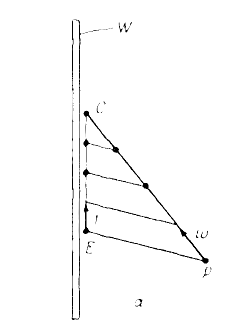
\includegraphics[width=0.8\textwidth]{wall.png}
	\caption{Игра с непреодолимой стеной $W$}
\label{fig:wall-game}
	\end{figure}
	Не ограничивая общности проведения игры будем считать что начальное положение E будет являться какой то точкой на W. В качестве платы также остается время захвата. 
	Если считать что для E лучше всего всегда оставаться около стены. Тогда у E есть выбор двигаться вдоль стены в одну или в другую сторону. Тогда P выбирает прямолинейную траекторию которая захватывает E в какой то точке С причем угол для прямой PE будет постоянным.
	\begin{figure}[H]
		\centering
		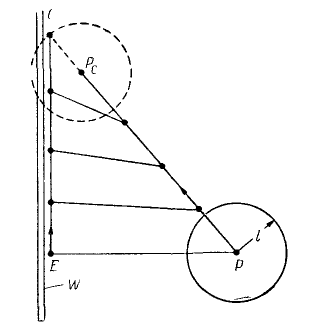
\includegraphics[width=0.8\textwidth]{rasseivayshie_poverhnosti.png}
	\caption{Курс столкновения в игре со стеной}
\label{fig:wall-dispersal-surface}
	\end{figure}
	Если же первоначально PE перпендикулярна W, тогда возникает дилемма в какую сторону стоит двигаться E и P соответсвенно. В каждый момент времени E может также поменять направление движения если P движется по траектории не меняя угол. Курс столкновения приводит E в некоторую точку C, а P в точку $P_c$ лежащую на отрезке CP и такая что $|CP_c| = l$ где l - радиус захвата. В течение развития игры наклон отрезка PE меняется. Отрезок становится менее горизонтальным, пока не превращается в $P_cC$
	Перейдя на динамику движения вдоль поверхности W, ясно, что редуцированное пространство здесь можно сделать двумерным с координатами x, y. Тогда уравнения движения выглядят так:
	\[\dot{x} = - w \cos\phi\]
	\[\dot{y} = \psi - w\sin\phi\]	
	где w > 1 и $-1 \leq \psi \leq 1$. Тогда основное уравнение:
	\[\min_{\phi}\max_{\psi} [-w(V_x\cos\phi + V_y\sin\phi) + V_y\psi] + 1 = 0.\] Стандартный прием $\rho = \sqrt{V_x^2 + V_y^2}$ получим $\cos \overline{\phi} = \frac{V_x}{\rho}, \ \ \ \sin \overline{\phi} = \frac{V_y}{\rho}$
	$\overline \psi = \operatorname{sgn}V_y$, и основное уравнение принимает вид $-w\rho + |V_y| + 1 = 0$. Уравнения характеристик в регрессивной форме: 
	\begin{equation*}
		\begin{cases}
			\dot{x} = w\frac{V_x}{\rho} \ \ \ \dot{V_x} = 0\\
			\dot{y} = -\operatorname{sgn}(V_y) + w\frac{V_y}{\rho}\ \ \ \dot{V_y} = 0
		\end{cases}
	\end{equation*}
	Также принимая терминальную поверхность в виде круга получим:
	\[x = l\cos s\]
	\[y = l\sin s\]
	\[V_s = 0 = l(-V_x\sin s + V_y\cos s)\]
	Решение будет в виде:
	\[V_x = \lambda \cos s, \ \ \ V_y = \lambda \sin s \]
Подставляя в основное уравнение, получаем $-w\lambda + \lambda|\sin s| + 1 = 0$, т.\,е. $\lambda = 1/(w - |\sin s|) > 0$ при $w > 1$; следовательно, вся окружность захвата является допустимой частью.
	Так как вектор градиента должен быть направлен внутрь, то $\lambda > 0$, тогда $\operatorname{sgn}V_y = \operatorname{sgn} s$ так как $\dot V_i = 0$ $V_i$ сохраняет одинаковое значение тогда получаем уравнение оптимальных траекторий 
	\[x = (l + w\tau)\cos s\]
	\[y = (l + w\tau)\sin s - \operatorname{sgn} s\, \tau\]
	
	\subsection{Отделение рассеивающих поверхностей}
	
	Пересечение траекторий двух классов, для которых цена игры совпадает для обеих траекторий и будет называться рассеивающей поверхностью. Фактически траектории - отрезки между терминальной и рассеивающей поверхностью. Рассмотрим найденные в прошлой главе траектории для s > 0 и для s < 0. Как раз эти траектории и дадут нам эти 2 класса, причем цена которая будет равна $\tau$ будет иметь одинаковое значение для обеих траекторий.
	
	\begin{figure}[H]
		\centering
		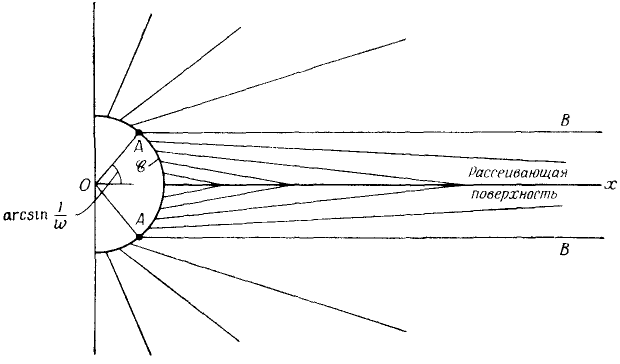
\includegraphics[width=0.8\textwidth]{otdeleniey_povehnostei.png}
	\caption{Траектории двух классов и рассеивающая поверхность $y = 0$}
\label{fig:separating-surface}
	\end{figure}
	
	Можно сказать что рассеивающая поверхность удовлетворяет уравнениям:
	\begin{equation*}
		\begin{cases}
			x = (l + w\tau)\cos{s_1} = (l + w\tau)\cos{s_2}\\
			y = (l + w\tau)\sin{s_1} - \tau = (l + w\tau)\sin{s_2} + \tau
		\end{cases}
	\end{equation*}
	т.к |$s_1$| $\leq$ $\frac{\pi}{2}$ =>$s_1 = -s_2 = s$ => y = 0. Получается что ось x, где x > l является рассеивающей поверхностью.
	\section{Численное построение функции платы}\label{sec:numeric}
	
	В предыдущих разделах была получена редуцированная система для игры
	<<шофёр--убийца>>. После перехода в систему координат, связанную с
	автомобилем, состояние игры описывается двумя переменными $x$ и $y$.
	Здесь $x$ и $y$ задают положение убегающего относительно шофёра в
	редуцированном пространстве.
	
	Редуцированная динамика имеет вид
	\[
	\dot{x}
	=
	-\frac{w_1}{R}y\varphi+w_2\sin\psi,
	\]
	\[
	\dot{y}
	=
	\frac{w_1}{R}x\varphi-w_1+w_2\cos\psi.
	\]
	Здесь $w_1$~--- скорость шофёра, $w_2$~--- скорость убегающего,
	$R$~--- минимальный радиус поворота автомобиля, $\varphi$~--- управление
	шофёра, а $\psi$~--- управление убегающего.
	
	В данной работе в качестве платы рассматривается время до захвата.
	Поэтому интегральная плотность платы принимается равной
	\[
	G(x,\varphi,\psi)\equiv 1.
	\]
	Терминальное множество задаётся условием
	\[
	x^2+y^2\leq l^2,
	\]
	где $l$~--- радиус захвата. При попадании состояния в это множество игра
	считается оконченной, поэтому функция платы удовлетворяет граничному
	условию
	\[
	V(x,y)=0,
	\qquad
	x^2+y^2\leq l^2.
	\]
	
	Вне области захвата функция платы должна удовлетворять уравнению
	Гамильтона--Якоби--Айзекса:
	\[
	\min_{\varphi}\max_{\psi}
	\left[
	V_x\left(
	-\frac{w_1}{R}y\varphi+w_2\sin\psi
	\right)
	+
	V_y\left(
	\frac{w_1}{R}x\varphi-w_1+w_2\cos\psi
	\right)
	+1
	\right]
	=0.
	\]
	Данное уравнение задаёт принцип оптимальности: шофёр выбирает управление
	$\varphi$, минимизирующее значение платы, а убегающий выбирает управление
	$\psi$, максимизирующее это значение.
	
	\subsection{Метод решения}

	Для численного решения уравнения Гамильтона--Якоби--Айзекса используется \emph{полностью дискретная полулагранжева схема} (semi-Lagrangian scheme) Барди--Фальконе--Соравиа~\cite{bfs,ff}. Она основана на дискретном принципе динамического программирования: цена в узле сетки равна минимаксу по управлениям от суммы <<время шага плюс цена в точке, куда приводит шаг>>. Значения функции цены между узлами восстанавливаются билинейной интерполяцией. Получающееся сеточное уравнение имеет вид неподвижной точки нелинейного оператора и решается \emph{методом итераций по значению} (value iteration) в варианте Якоби. Сходимость таких схем к вязкостному решению уравнения Айзекса при $h,\tau\to 0$ доказана в~\cite{bfs,bcd}.

	\subsection{Сеточная аппроксимация}

	Расчётная область $[-L,L]^2$ покрывается равномерной сеткой
	\[
	x_i=-L+ih,\qquad y_j=-L+jh,\qquad i,j=0,\dots,n-1,\qquad n=\frac{2L}{h}+1 .
	\]
	Функция платы заменяется сеточной функцией $V_{ij}\approx V(x_i,y_j)$. Множества управлений заменяются конечными наборами
	\[
	\Phi=\{-1,0,1\},\qquad \Psi=\Bigl\{\psi_k=\frac{2\pi k}{24},\ k=0,\dots,23\Bigr\}.
	\]
	Набора $\Phi$ достаточно, так как гамильтониан линеен по $\varphi$ и минимум достигается на концах отрезка $[-1,1]$; значение $\varphi = 0$ нужно на универсальных линиях.

	Для узла $z=(x,y)$ и пары управлений $(\varphi,\psi)$ точка, в которую система переходит за время $\tau$, равна
	\[
	z^{+}=z+\tau f(z,\varphi,\psi),\qquad
	f=\Bigl(-\frac{w_1}{R}y\varphi+w_2\sin\psi,\ \ \frac{w_1}{R}x\varphi-w_1+w_2\cos\psi\Bigr).
	\]
	Значение $V(z^{+})$ вычисляется билинейной интерполяцией по четырём соседним узлам. Внутри круга захвата оно полагается равным нулю, вне расчётной области --- равным $T_{\max}$.

	\paragraph{Выбор шага по времени.} Шаг $\tau$ согласуется с шагом сетки:
	\[
	\tau=\frac{h}{w_1+w_2},
	\]
	т.\,е. вблизи круга захвата точка за один шаг смещается примерно на одну ячейку. Для полулагранжевой схемы с линейной интерполяцией локальная погрешность в областях гладкости имеет порядок $O(\tau+h^2/\tau)$~\cite{ff}, поэтому при $\tau\sim h$ получается порядок $O(h)$. Если же $\tau$ фиксировать, а сетку измельчать, ошибка интерполяции $h^2/\tau$ накапливается за большое число мелких шагов, и уточнения не происходит.

	\paragraph{Ограничение $T_{\max}$.} Если из некоторого положения убегающий может уклоняться от захвата сколь угодно долго, точная цена бесконечна. Кроме того, траектории, выходящие за пределы расчётной области, обрываются. Поэтому значения ограничиваются сверху величиной $T_{\max}$: значение $V=T_{\max}$ означает, что за время $T_{\max}$ захват не гарантирован (или не может быть установлен в пределах расчётной области). В расчётах $T_{\max}=100$, что заведомо больше времени захвата в рассматриваемой части плоскости.

	\subsection{Итерационная схема}

	Если отрезок $[z,z^{+}]$ пересекает круг захвата $x^2+y^2\le l^2$, то шаг завершает игру. Обозначим через $\theta\in[0,1]$ долю шага до первого пересечения (наименьший корень квадратного уравнения $|z+\theta(z^{+}-z)|^2=l^2$). Тогда стоимость перехода
	\[
	Q(z,\varphi,\psi)=
	\begin{cases}
		\tau\theta, & \text{если отрезок } [z,z^{+}] \text{ пересекает круг захвата},\\
		\tau+V^{old}(z^{+}) & \text{иначе}.
	\end{cases}
	\]
	Проверка всего отрезка, а не только его конца, нужна, чтобы шаг не <<перескакивал>> круг захвата.

	Начальное приближение: $V_{ij}=0$ внутри круга захвата и $V_{ij}=T_{\max}$ вне его. Для каждого узла вне круга захвата выполняется обновление
	\[
	V^{new}_{ij}=\min\Bigl\{T_{\max},\ \min_{\varphi\in\Phi}\ \max_{\psi\in\Psi} Q(z_{ij},\varphi,\psi)\Bigr\}.
	\]
	Итерации продолжаются, пока невязка $\max_{ij}|V^{new}_{ij}-V^{old}_{ij}|$ не станет меньше $\varepsilon=10^{-4}$.

	Веса билинейной интерполяции неотрицательны, а операции $\min$ и $\max$ монотонны. Поэтому оператор схемы монотонен, значения итераций остаются в $[0,T_{\max}]$ при любом $\tau$, а последовательность приближений, начинающаяся с $T_{\max}$, монотонно не возрастает и сходится.

	\subsection{Оптимальные управления}

	Управления для автоматической игры берутся из того же дискретного минимакса, по которому построена функция цены. В точке $z$ для каждого $\varphi\in\Phi$ находится худшее для шофёра направление убегающего
	\[
	\psi^{*}(\varphi)=\arg\max_{\psi} Q(z,\varphi,\psi),
	\]
	после чего шофёр выбирает $\varphi^{*}=\arg\min_{\varphi}Q\bigl(z,\varphi,\psi^{*}(\varphi)\bigr)$, а убегающий --- $\psi^{*}(\varphi^{*})$ (для синтеза используется 72 направления $\psi$). Формулы $\varphi^{*}=-\operatorname{sgn}(xV_y-yV_x)$ и $\sin\psi^{*}=V_x/\sqrt{V_x^2+V_y^2}$, $\cos\psi^{*}=V_y/\sqrt{V_x^2+V_y^2}$ справедливы там, где $V$ гладкая. На барьере и рассеивающих линиях градиент не определён, и численное дифференцирование даёт неверные управления; минимакс по сеточной функции этого недостатка не имеет.

	\subsection{Результаты расчётов}

	Параметры игры: $w_1=120$, $w_2=100$, $R=60$, $l=35$. Радиус поворота выбран так, чтобы выполнялось условие Айзекса~\cite{isaacs}, при котором захват гарантирован из любого положения:
	\[
	\frac{l}{R}>\sqrt{1-\gamma^2}+\arcsin\gamma-1,\qquad \gamma=\frac{w_2}{w_1}.
	\]
	При $\gamma=5/6$ правая часть равна $\approx 0{,}54$, а $l/R\approx 0{,}58$. (При $R=120$ условие нарушается: $l/R\approx 0{,}29$, и из большей части плоскости убегающий уходит от захвата, т.\,е. $V=\infty$.)

	Расчётная область $L=600$, $T_{\max}=100$, $\varepsilon=10^{-4}$. Расчёты выполнены на трёх сетках (табл.~\ref{tab:runs}). Реализация на NumPy с предвычисленной таблицей переходов совпадает с базовой реализацией на Python до ошибок округления.

	Для проверки точности используется случай, когда убегающий находится прямо по курсу шофёра ($x=0$, $y>l$): обоим игрокам выгодно двигаться по прямой, и время захвата известно точно,
	\[
	V(0,y)=\frac{y-l}{w_1-w_2}.
	\]

	\begin{table}[H]
		\centering
		\caption{Расчёты на последовательности сеток ($L=600$)}
		\label{tab:runs}
		\small
		\begin{tabular}{rrrrrrr}
			\hline
			$h$ & $\tau$ & сетка & итераций & время, с & ошибка на оси $x=0$ & $\overline{|V_h-V_{2h}|}$ \\
			\hline
			20 & 0{,}0909 & $61\times61$ & 1872 & 8 & 7{,}80 & --- \\
			10 & 0{,}0455 & $121\times121$ & 2645 & 63 & 2{,}45 & 4{,}35 \\
			5 & 0{,}0227 & $241\times241$ & 3896 & 464 & 0{,}11 & 1{,}49 \\
			\hline
		\end{tabular}
	\end{table}
	В столбце <<ошибка на оси>> --- максимальное отклонение от точного значения $V(0,y)$ при $60\le y\le 300$, в последнем столбце --- средняя разность решений на соседних сетках в окне $|x|\le 200$, $-150\le y\le 250$. Обе величины уменьшаются при измельчении сетки; на самой мелкой сетке ошибка на оси составляет около 1\,\% от значения.

	\begin{figure}[H]
		\centering
		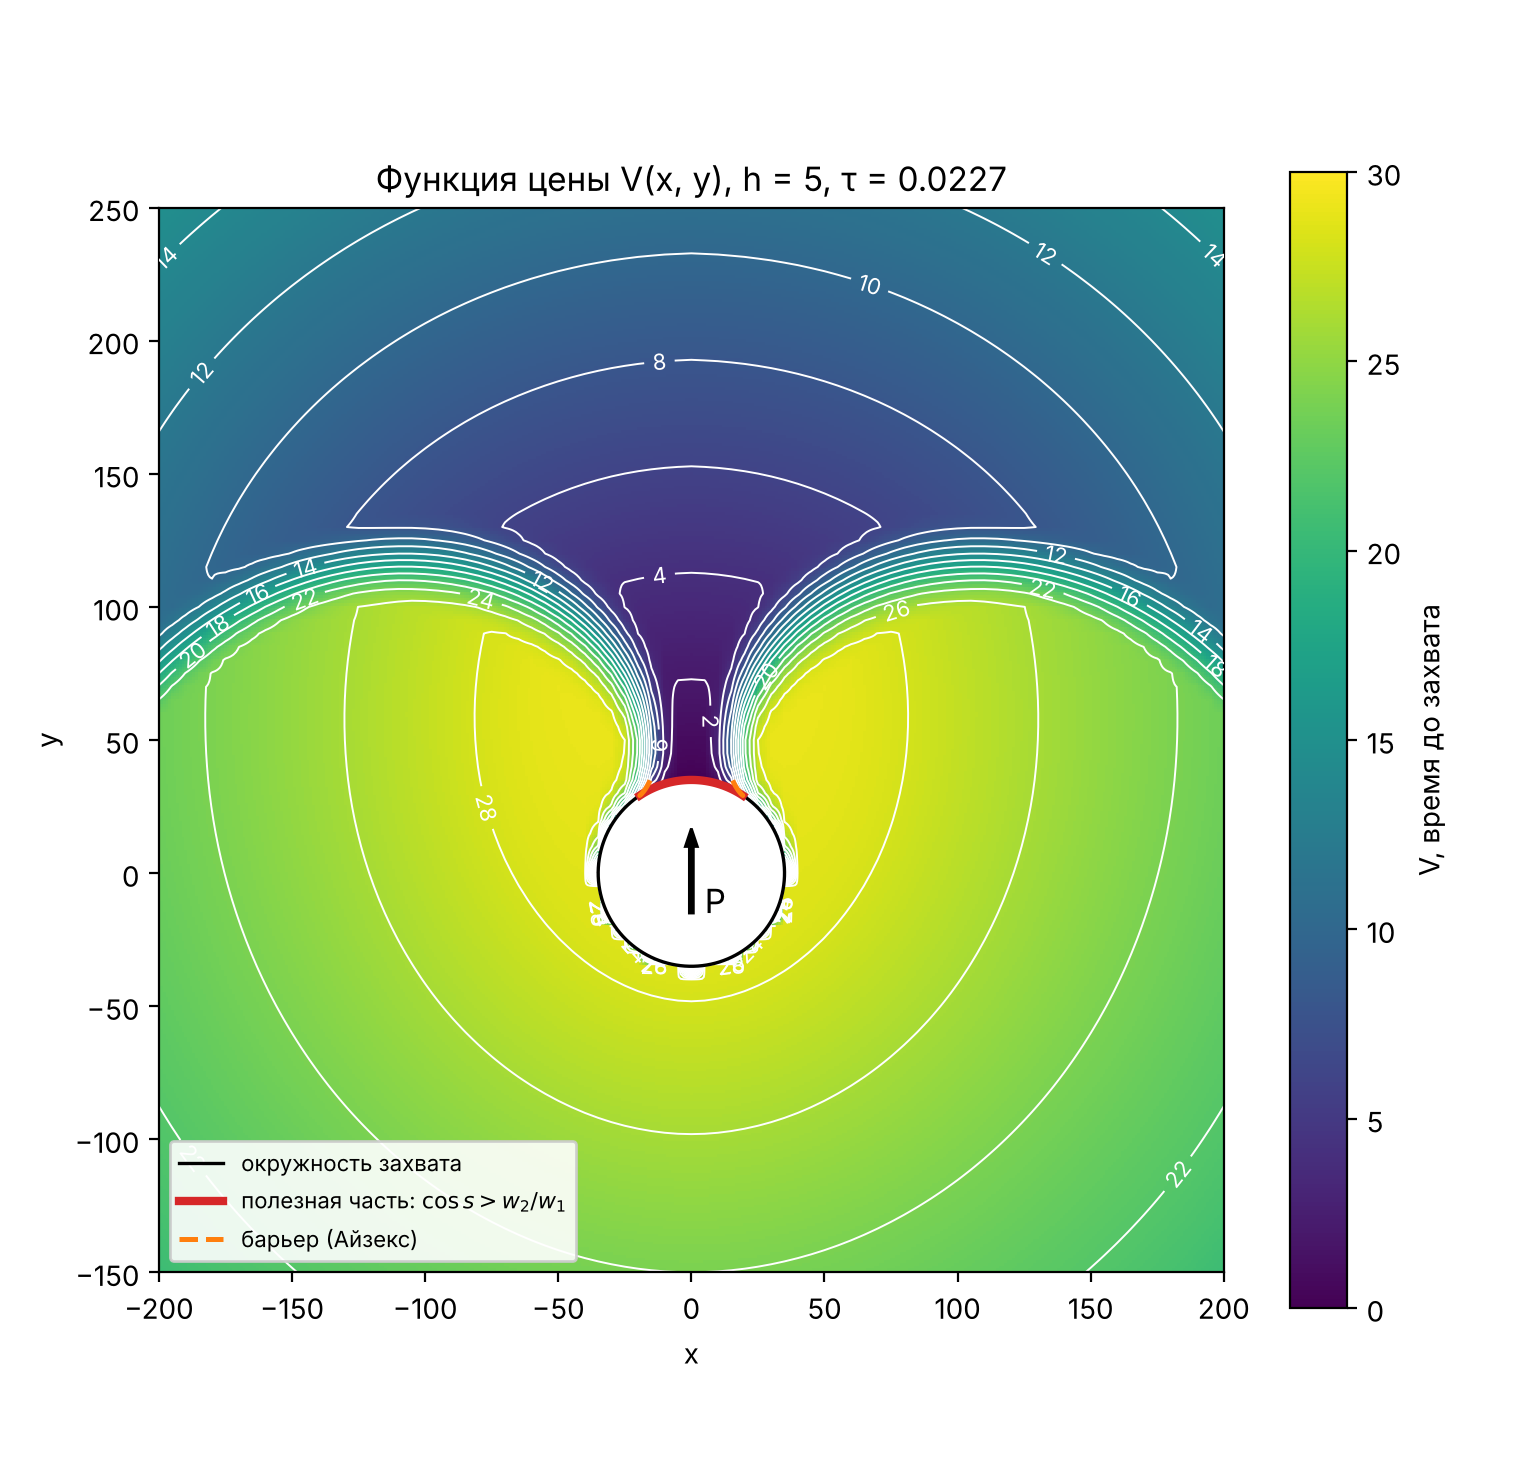
\includegraphics[width=0.85\textwidth]{v_heatmap.png}
		\caption{Функция цены $V(x,y)$ ($h=5$): тепловая карта и линии уровня. Красным выделена допустимая часть окружности захвата $\cos s>w_2/w_1$, пунктиром --- начальные участки барьера Айзекса}
		\label{fig:v-heatmap}
	\end{figure}

	\begin{figure}[H]
		\centering
		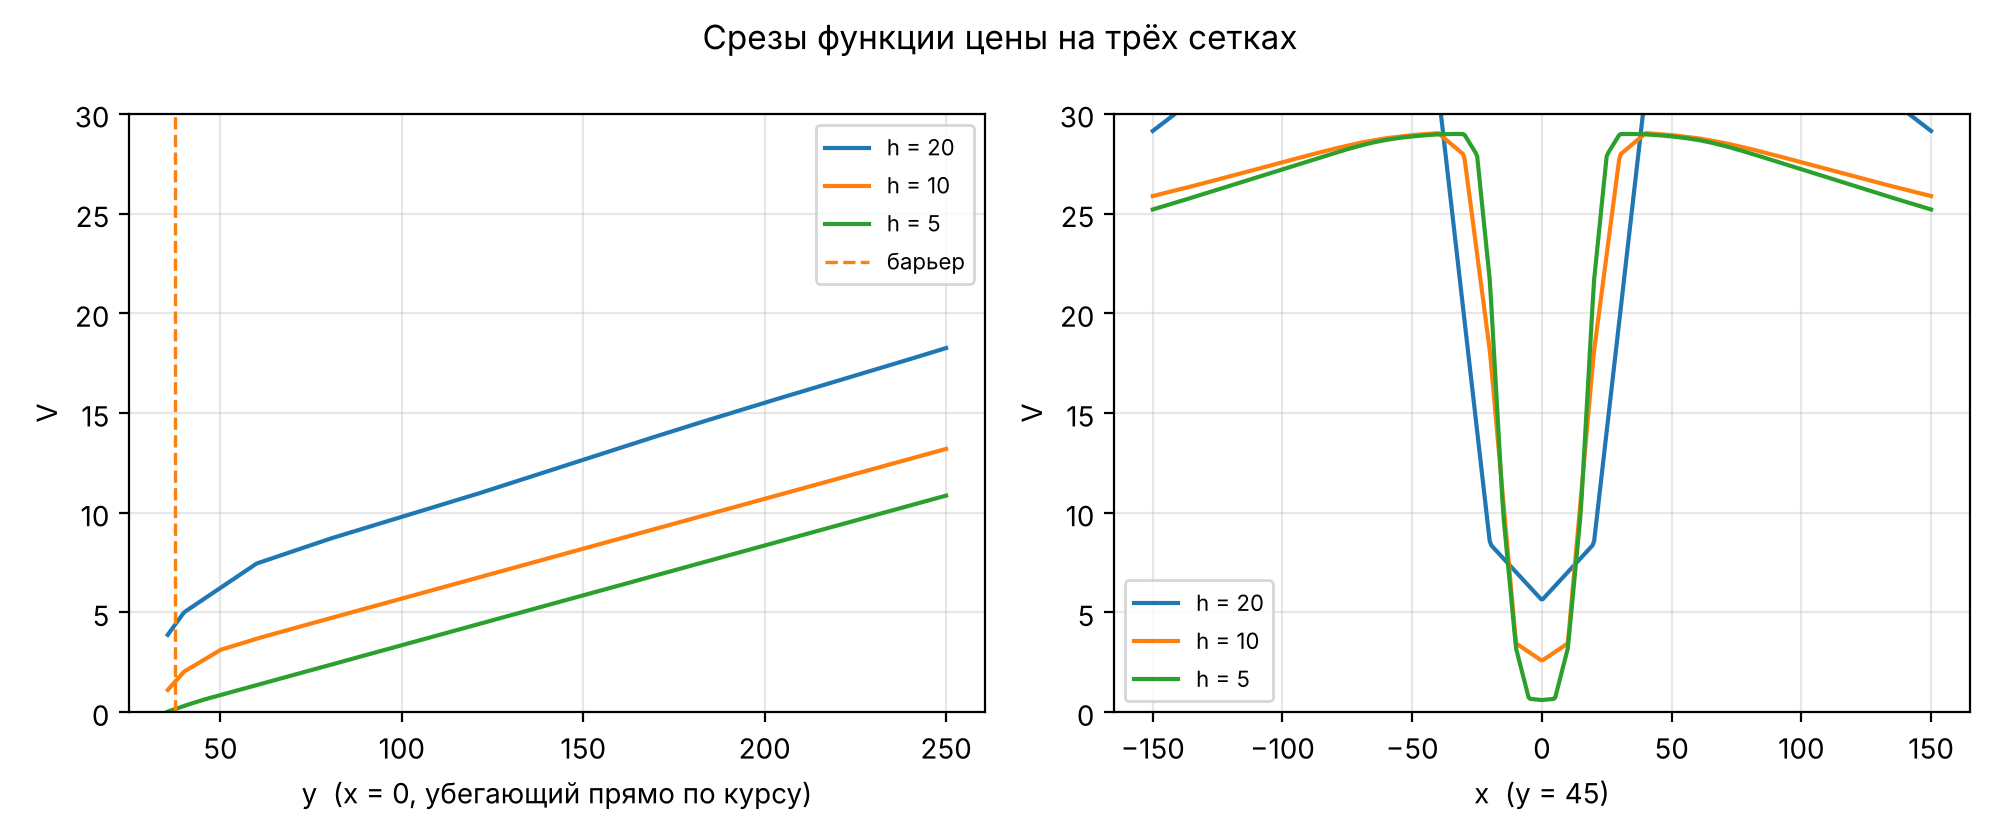
\includegraphics[width=\textwidth]{v_slices.png}
		\caption{Срезы функции цены на трёх сетках: вдоль оси $y$ (убегающий прямо по курсу шофёра) и вдоль прямой $y=45$}
		\label{fig:v-slices}
	\end{figure}

	\begin{figure}[H]
		\centering
		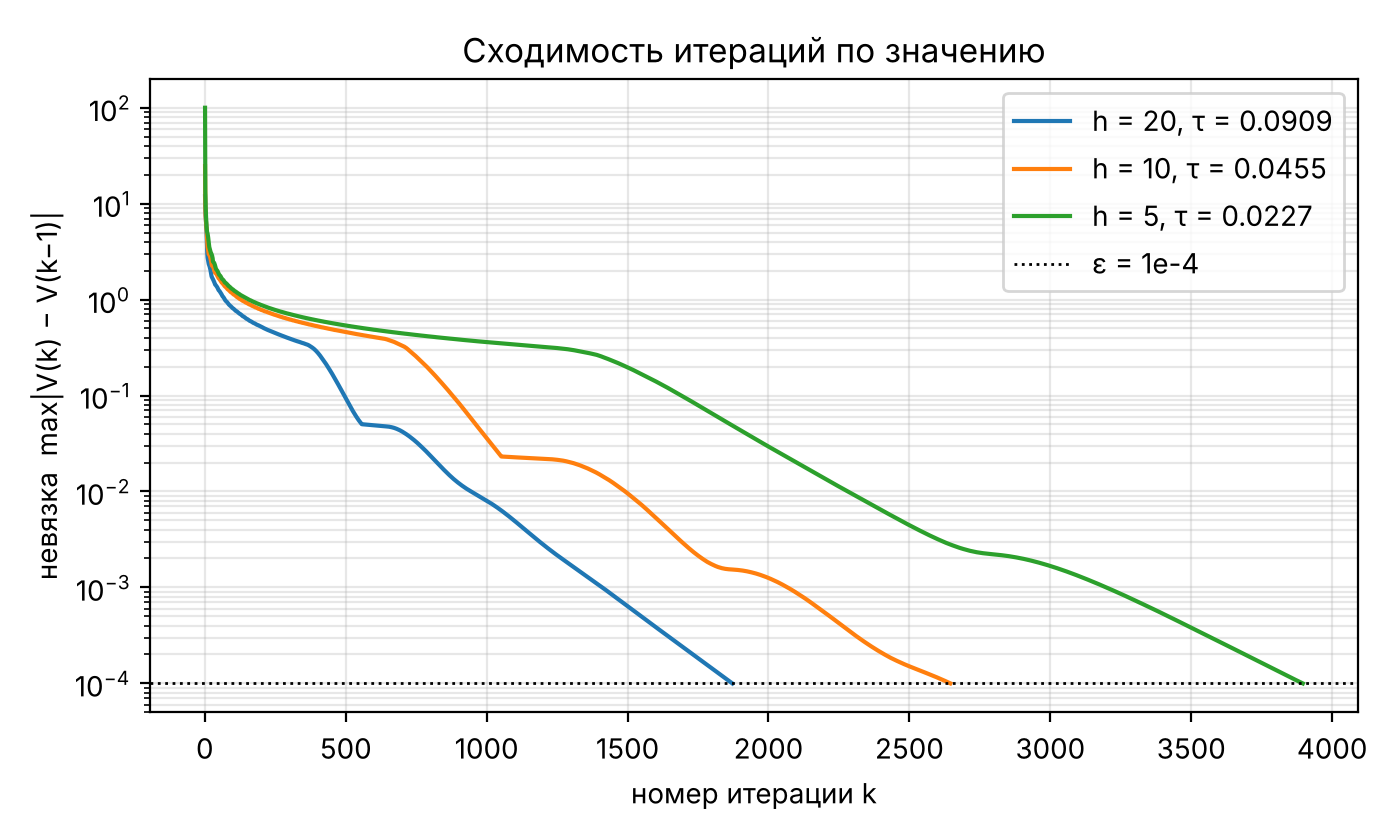
\includegraphics[width=0.85\textwidth]{v_convergence.png}
		\caption{Сходимость итераций по значению: невязка в зависимости от номера итерации}
		\label{fig:v-convergence}
	\end{figure}

	\subsection{Интерпретация результатов}

	Функция цены показывает приближённое время до захвата при оптимальном поведении игроков. Малые значения соответствуют положениям, из которых шофёр быстро достигает захвата, большие --- положениям, из которых убегающий дольше уклоняется.

	Наименьшие значения сосредоточены в узкой области прямо перед шофёром, которая опирается на допустимую дугу окружности захвата (рис.~\ref{fig:v-heatmap}). Если убегающий находится сбоку или сзади, шофёру приходится разворачиваться, и время захвата составляет около 25--30~с. Области <<впереди>> и <<сбоку>> разделены линиями, на которых линии уровня сгущаются: это линии разрыва функции цены (барьер), по разные стороны которых оптимальные траектории принципиально различны. На сеточном решении разрыв <<размазан>> на несколько ячеек; при измельчении сетки переход становится всё круче (рис.~\ref{fig:v-slices}, справа).

	Несимметричность графиков по оси $y$ объясняется самой редуцированной динамикой: слагаемое $-w_1$ в уравнении для $\dot y$ выделяет направление движения автомобиля. Положения впереди и позади шофёра имеют разный смысл. Симметрия относительно оси $y$ ($V(x,y)=V(-x,y)$) следует из инвариантности динамики относительно замены $(x,\varphi,\psi)\to(-x,-\varphi,-\psi)$. Подробный обзор структуры решения этой игры приведён в~\cite{pt}.

	Число итераций растёт при уменьшении шага $\tau$ (рис.~\ref{fig:v-convergence}), так как за одну итерацию информация от круга захвата распространяется лишь на один шаг по времени. Уменьшить число итераций можно методом Гаусса--Зейделя или преобразованием Кружкова $v=1-e^{-V}$, которое делает оператор сжимающим.

	\section{Игра в прямоугольной арене}\label{sec:arena}

	\subsection{Постановка}

	В программной модели игроки движутся не по всей плоскости, а внутри прямоугольной арены $0\le X\le 800$, $0\le Y\le 600$, ограниченной четырьмя стенами с углами. Стены непреодолимы: если шаг выводит игрока за границу, его координаты проектируются на арену, т.\,е. составляющая скорости, направленная в стену, гасится, а касательная сохраняется. Управления и скорости игроков те же, что в разделе~\ref{sec:numeric}.

	Редукция к двум координатам $(x,y)$ здесь, строго говоря, неприменима. Положение стен относительно шофёра зависит от его абсолютных координат и курса $\theta$, поэтому полное состояние игры в арене пятимерно: $(X_P,Y_P,\theta,X_E,Y_E)$. Расчёт функции цены на сетке по пяти переменным требует очень грубой дискретизации и не использовался. Вместо этого стены учитываются приближённо, а функция цены берётся из редуцированной задачи --- той же двумерной сетки $V(x,y)$, построенной в разделе~\ref{sec:numeric}.

	\subsection{Стратегия с прогнозом}

	В каждый момент времени для каждой пары управлений $(\varphi,\psi)$, $\varphi\in\{-1,0,1\}$, $\psi\in\{2\pi k/36\}$, выполняется короткий прогноз (rollout): движение обоих игроков с постоянными управлениями на горизонте $H=0{,}3$~с с шагом $0{,}05$~с по уравнениям в абсолютных координатах и с упором в стены. После прогноза состояние переводится в редуцированные координаты и оценивается по сеточной функции цены:
	\[
	Q(\varphi,\psi)=
	\begin{cases}
		t_c+L, & \text{захват в момент } t_c\le H,\\
		H+L+V\bigl(x(H),y(H)\bigr), & \text{захвата нет}.
	\end{cases}
	\]
	Здесь $L$ --- время, <<потерянное>> шофёром из-за упора в стену: на каждом шаге прогноза к $L$ добавляется доля шага, на которую стена укоротила перемещение шофёра. Поправка нужна потому, что функция $V(x,y)$ о стенах не знает и считает, что шофёр всегда движется со скоростью $w_1$.

	\paragraph{Прогноз убегающего.} Горизонта $H=0{,}3$~с убегающему мало: за это время он проходит лишь 30 единиц и <<не видит>> стену, к которой бежит, а функция $V(x,y)$ о стенах не знает. Поэтому направления убегающего оцениваются более длинным прогнозом: после первых $H$ секунд он ещё $T_E=2$~с сохраняет выбранное направление (скользя вдоль стен, если упирается в них), а шофёр в это время поворачивает в сторону убегающего (базовая стратегия преследования). Полученную оценку обозначим $Q_E(\varphi,\psi)$; ответ убегающего на управление шофёра
	\[
	\psi_E(\varphi)=\arg\max_{\psi}Q_E(\varphi,\psi).
	\]
	Если направление ведёт в стену, убегающий упирается в неё, шофёр за время прогноза приближается, и оценка $Q_E$ оказывается малой --- такое направление отбрасывается.

	\paragraph{Выбор управлений.} Шофёр выбирает управление, наилучшее против этого ответа убегающего:
	\[
	\varphi^{*}=\arg\min_{\varphi}Q\bigl(\varphi,\psi_E(\varphi)\bigr),\qquad \psi^{*}=\psi_E(\varphi^{*}).
	\]
	Такая схема --- одношаговое улучшение базовых стратегий с прогнозом (rollout) и терминальной оценкой по функции цены редуцированной игры. Дополнительно используются два правила, исключающие <<застревание>> шофёра у стены: при почти равных оценках сохраняется прежнее $\varphi$, а если шофёр упирается в стену (курс направлен наружу у границы), он продолжает поворот с максимальной кривизной в ту же сторону, пока не освободится.

	Сетка $V(x,y)$ для арены рассчитывается один раз и хранится в файле: $h=10$, $L=1100$ (относительное расстояние в арене не превышает $1000$), $T_{\max}=100$, сходимость за 3418 итераций. Выбор управлений в игре занимает около 4~мс, что позволяет пересчитывать их на каждом шаге моделирования ($0{,}02$~с).

	\subsection{Результаты моделирования}

	Моделирование проводилось для 200 случайных начальных положений (расстояние между игроками не меньше 150, курс шофёра случайный) с шагом $0{,}02$~с и ограничением времени 60~с. Для сравнения использовались простые стратегии: <<преследование>> --- шофёр поворачивает с максимальной кривизной в сторону убегающего, <<бегство>> --- убегающий движется прямо от шофёра.

	\begin{table}[H]
		\centering
		\caption{Время захвата в арене, 200 случайных стартов}
		\label{tab:arena}
		\small
		\begin{tabular}{llrrrr}
			\hline
			Шофёр & Убегающий & захватов & среднее, с & максимум, с & E у стены \\
			\hline
			по $V(x,y)$ & по $V(x,y)$ & 200 & 7{,}56 & 48{,}7 & 49 \\
			преследование & по $V(x,y)$ & 200 & 5{,}35 & 9{,}4 & 71 \\
			по $V(x,y)$ & бегство & 200 & 5{,}87 & 10{,}6 & 200 \\
			преследование & бегство & 200 & 5{,}66 & 8{,}7 & 200 \\
			\hline
		\end{tabular}
	\end{table}
	В последнем столбце --- число партий, в которых в момент захвата убегающий находился ближе 25 к стене, т.\,е. был к ней прижат.

	\begin{figure}[H]
		\centering
		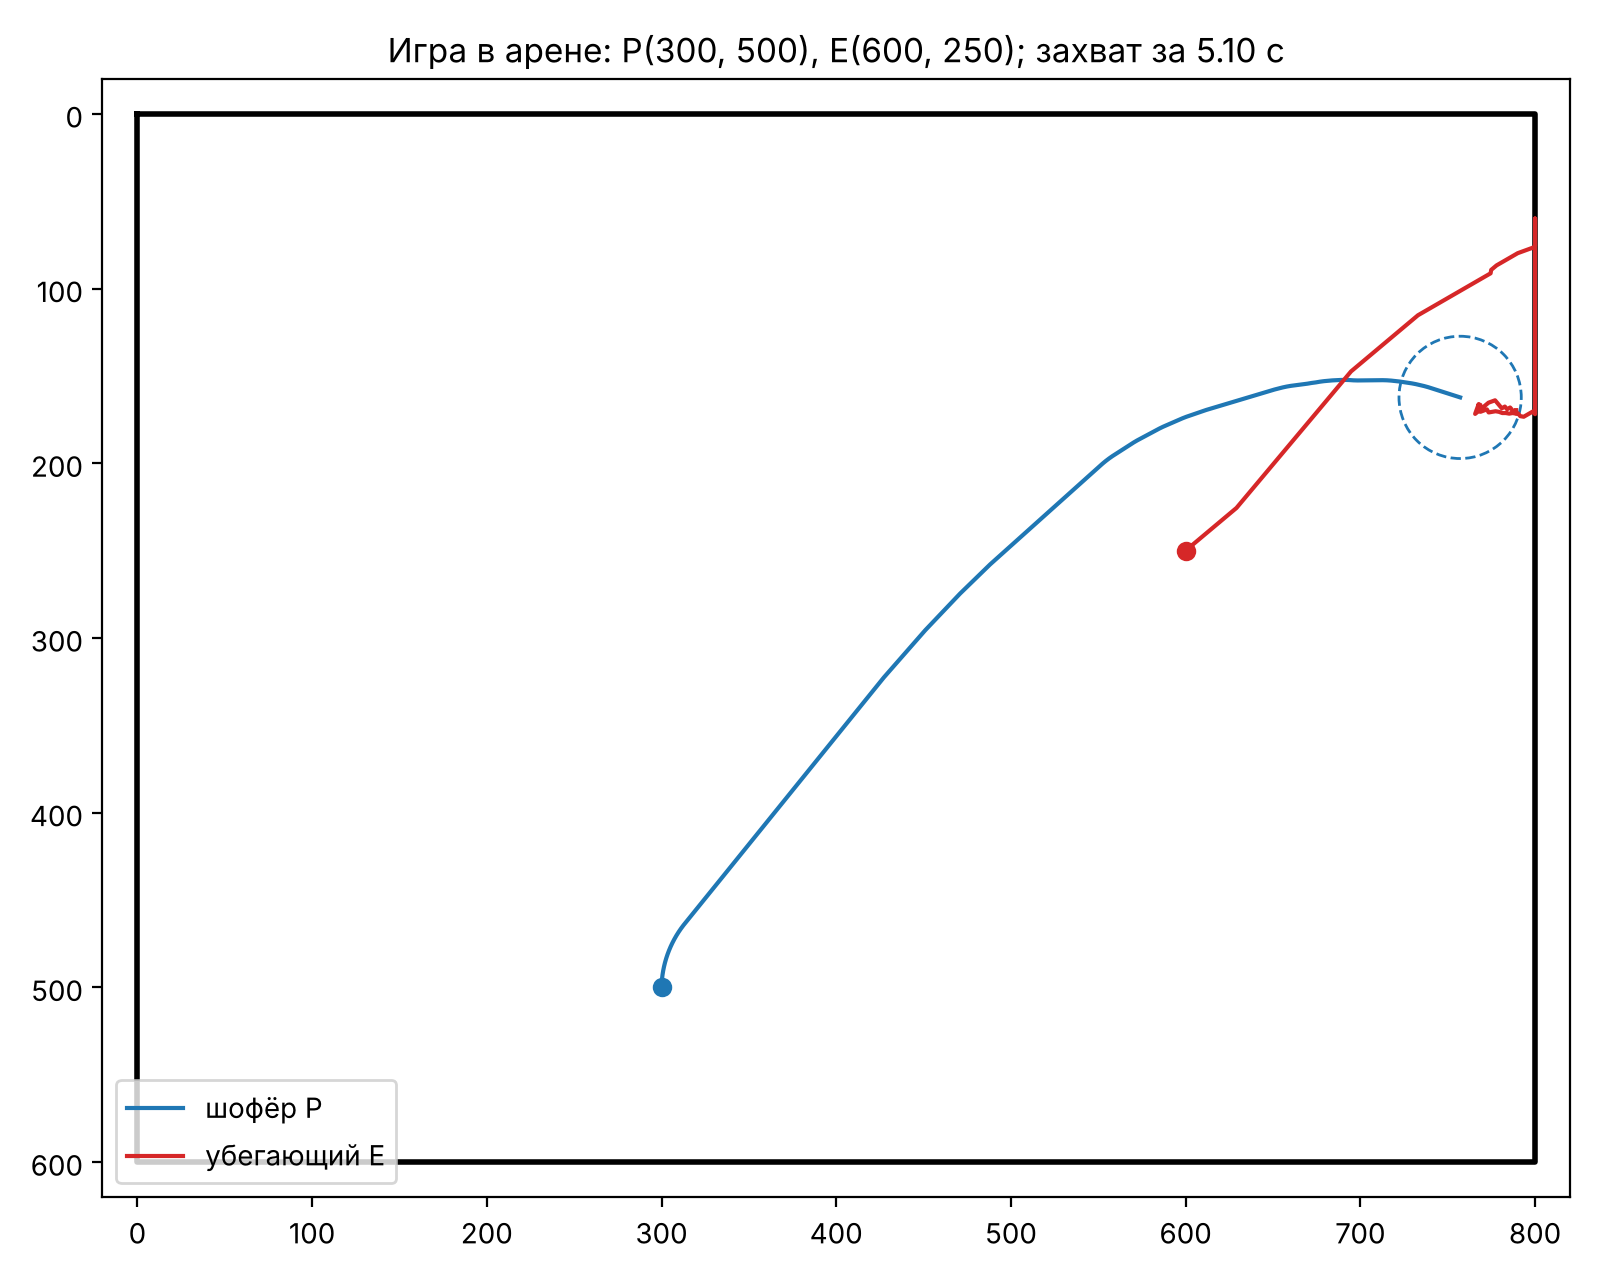
\includegraphics[width=0.8\textwidth]{arena_trajectory.png}
		\caption{Траектории игроков в арене при стратегиях по $V(x,y)$: старт $P(300,500)$, $E(600,250)$}
		\label{fig:arena-traj}
	\end{figure}

	\begin{figure}[H]
		\centering
		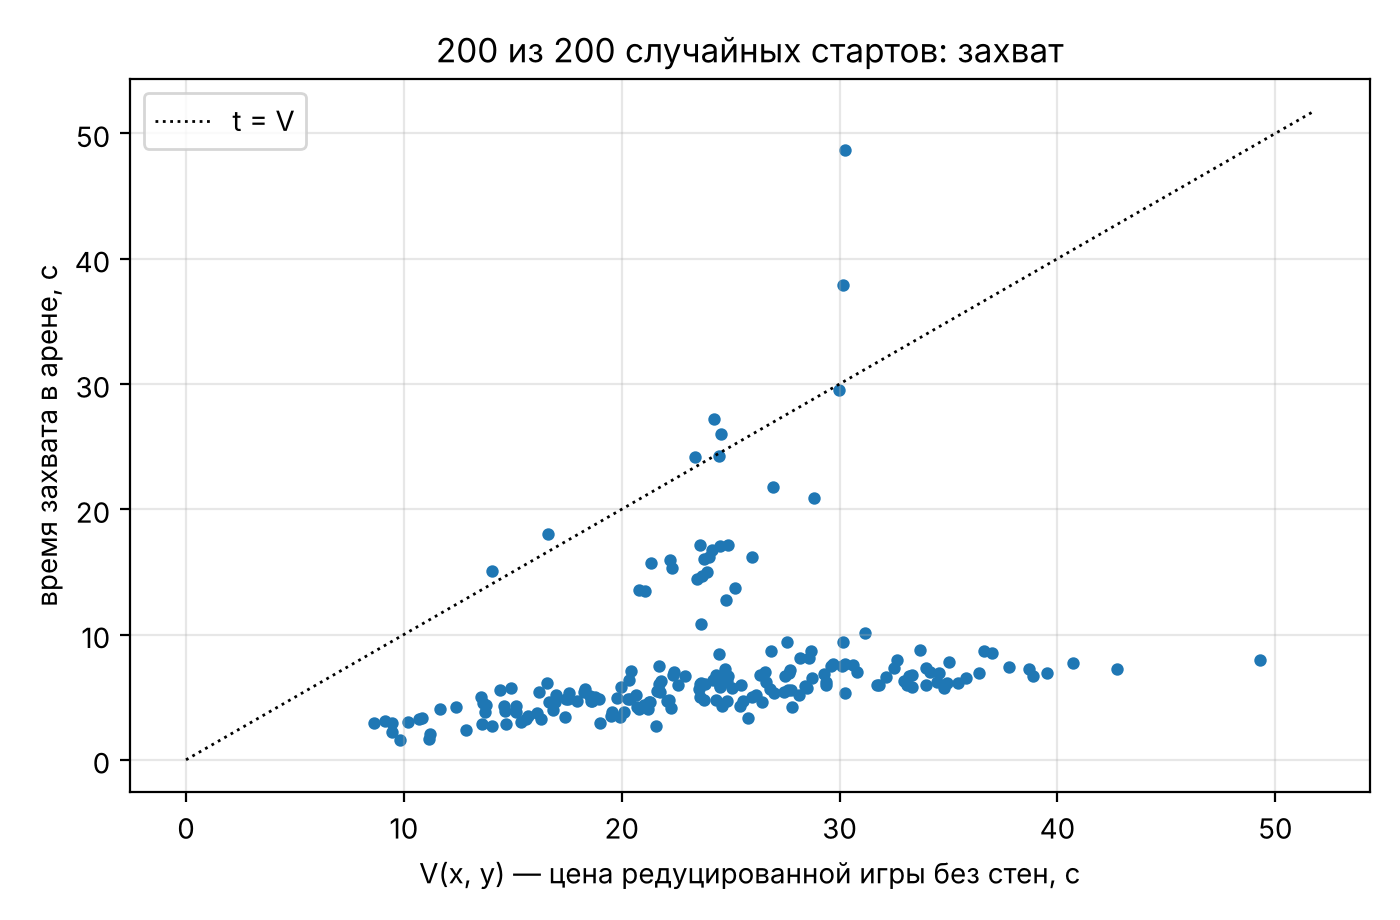
\includegraphics[width=0.8\textwidth]{arena_times.png}
		\caption{Время захвата в арене в сравнении с ценой $V(x,y)$ редуцированной игры без стен для тех же начальных положений}
		\label{fig:arena-times}
	\end{figure}

	Во всех партиях захват произошёл. Время захвата в арене (в среднем 5--8~с) существенно меньше цены редуцированной игры без стен для тех же начальных положений (10--50~с, рис.~\ref{fig:arena-times}): стены лишают убегающего возможности уходить по прямой.

	Без длинного прогноза убегающий, ориентируясь только на $V(x,y)$, бежал прочь от шофёра прямо в стену и в 93 партиях из 100 (отдельный прогон на первых 100 стартах) был пойман прижатым к ней. С прогнозом $T_E=2$~с он заранее сворачивает вдоль стены: против шофёра со стратегией по $V(x,y)$ он прижат к стене лишь в 49 партиях из 200 и держится в среднем 7{,}56~с против 5{,}87~с при простом бегстве (при простом бегстве он прижат к стене во всех партиях).

	Простое преследование ловит убегающего быстрее, чем стратегия по $V(x,y)$ (табл.~\ref{tab:arena}). Это ожидаемо: функция цены редуцированной игры оптимальна для плоскости без стен и не учитывает, что стены сами ограничивают убегающего, а прогноз учитывает стены лишь на несколько секунд вперёд. Точное оптимальное поведение в арене требует функции цены по полному пятимерному состоянию; предложенная стратегия --- приближённая, но использует только двумерную сетку и работает в реальном времени.

	\section{Заключение}
	
	В данной работе была рассмотрена дифференциальная игра
	<<шофёр--убийца>>, в которой преследователь движется с ограничением на
	радиус поворота, а убегающий выбирает направление своего движения. Была
	записана математическая модель движения игроков и выполнен переход к
	редуцированному пространству, где состояние игры описывается двумя
	переменными $x$ и $y$.
	
	На основе редуцированной модели была построена функция платы $V(x,y)$,
	которая показывает, насколько выгодным или невыгодным является данное
	относительное положение игроков. В качестве платы рассматривалось время
	до захвата, поэтому малые значения функции соответствуют положениям, из
	которых шофёр быстро догоняет убегающего, а большие значения соответствуют
	положениям, где убегающий может дольше уклоняться.
	
	Для численного построения функции платы была реализована полностью дискретная полулагранжева схема с итерациями по значению. Шаг по времени согласован с шагом сетки, захват проверяется на всём отрезке шага, а область, из которой захват не гарантирован, отделяется ограничением $T_{\max}$. Расчёты на последовательности сеток показали сходимость итераций и уменьшение ошибки при измельчении сетки; на оси, где цена известна точно, ошибка на самой мелкой сетке составляет около 1\,\%.

	Также была реализована автоматическая стратегия движения игроков в прямоугольной арене с четырьмя стенами. Она использует ту же двумерную сетку функции платы редуцированной игры, а стены учитывает коротким прогнозом движения с упором в стены; управления выбираются по минимаксу. Чтобы убегающий не упирался в стены, его направления оцениваются более длинным прогнозом. Моделирование 200 партий показало, что захват в арене происходит всегда и значительно быстрее, чем в игре без стен, а убегающий с прогнозом реже оказывается прижат к стене и держится дольше, чем при простом бегстве.

	Таким образом, в работе была построена и реализована численная модель
	игры <<шофёр--убийца>>, получена функция платы в редуцированном
	пространстве и показано, как её можно использовать для моделирования
	поведения игроков.
	
	\addcontentsline{toc}{section}{Список литературы}
	\begin{thebibliography}{9}
		\bibitem{isaacs} Айзекс Р. Дифференциальные игры. --- М.: Мир, 1967. --- 480~с.
		\bibitem{bfs} Bardi M., Falcone M., Soravia P. Fully discrete schemes for the value function of pursuit-evasion games~// Advances in Dynamic Games and Applications. Annals of the International Society of Dynamic Games, vol.~1. --- Boston: Birkhäuser, 1994.
		\bibitem{ff} Falcone M., Ferretti R. Semi-Lagrangian Approximation Schemes for Linear and Hamilton--Jacobi Equations. --- Philadelphia: SIAM, 2014.
		\bibitem{bcd} Bardi M., Capuzzo-Dolcetta I. Optimal Control and Viscosity Solutions of Hamilton--Jacobi--Bellman Equations. --- Boston: Birkhäuser, 1997.
		\bibitem{pt} Patsko V.\,S., Turova V.\,L. Homicidal chauffeur game: history and modern studies~// Advances in Dynamic Games. Annals of the International Society of Dynamic Games, vol.~11. --- Boston: Birkhäuser, 2011.
	\end{thebibliography}

\end{document}
